% Chapter Template

\chapter{Rețeaua Bayesiană} % Main chapter title

\label{Chapter2} % Change X to a consecutive number; for referencing this chapter elsewhere, use \ref{ChapterX}

%-----------------------------------
%	SECTION 1
%-----------------------------------
\section{Definiție}

O rețea Bayesiană este un model probabilistic grafic care reprezintă un set de variabile aleatoare și dependețele condiționale dintre ele sub forma unui graf orientat aciclic (DAG).

Fiecare nod al grafului reprezintă o variabilă aleatoare, iar arcele dintre noduri reprezintă dependențele probabilistice dintre nodurile conectate.

Clasificatorul naiv Bayes presupune că toate variabilele sunt independent condiționate, în contrast cu rețelele Bayesiene, care permite condiționarea independentă aplicată la subseturi de variabile.

Aceste modele probabilistice, ca modelul naiv Bayes sau modelele logistice de regresie sunt diferite de alte modele de reprezentare, cum ar fi arborii de decizie, prin faptul că produc estimări probabilistice în loc de clasificări exacte.

Pentru fiecare clasă de valori, estimează probabilitatea ca o instanță dată să aparțină acelei clase.
Aceste estimări probabilistice sunt mai utile decât simple predicții, deoarece pot fi clasate, iar costul acestora poate fi minimizat.

%-----------------------------------
%	SECTION 2
%-----------------------------------
\section{Deducția rețelei Bayesiene}

Deducția rețelei Bayesiene se realizează în 3 pași:
\begin{itemize}
\item Deducția de variabile neobservate; rețeaua poate fi folosită pentru a oferi informații probabilistice despre relațiile dintre variabile.
\item Învățarea probabilităților condiționale; pentru fiecare nod specificarea distribuției probabilităților condiționate de părinții nodului respectiv.
\item Învățarea structurii rețelei și construirea grafului.
\end{itemize}

%-----------------------------------
%	SECTION 3
%-----------------------------------
\section{Învățarea rețelei Bayesiene}

Algoritmul pentru construirea rețelei Bayesiene are două componente: o funcție pentru evaluarea rețelei în funcție de date și o metodă de a genera toate rețelele posibile și a o selecta pe cea mai bună.

După definirea structurii grafului care reprezintă rețeaua, calculul probabilităților condiționale este ușor de realizat, necesitând doar calculul frecvențelor relative a combinațiilor de atribute asociate din setul de date.

\subsection{Teorema lui Bayes}

Pentru a putea exprima în termeni matematici teorema lui Bayes, se folosesc anumite  notaţii.  Considerăm  o  ipoteză  h  din  spaţiul  ipotezelor  H.  Prin  P(h)  notăm probabilitatea iniţială a ipotezei h. Prin P(D) ne referim la probabilitatea anterioară observării datelor de antrenare D, iar la probabilitatea de a observa datele D în raport cu ipoteza h, prin P(D|h).  Deşi  trebuie  să  avem  în  vedere  toate  acestea,  în  lumea  maşinilor  de  învăţare  suntem interesaţi de o altă probabilitate notată prin P(h|D). Aceasta este probabilitatea ulterioară a lui h, aceea ca ipoteza h să se petreacă având în vedere datele de antrenare D. Aceasta reflectă influenţa datelor de antrenare  asupra decizilor care pot fi luate, în contrast cu P(h), probabilitate independent de D.

Teoremalui  Bayes furnizează metoda de a calcula probabilitatea ulterioară, P(h|D), din P(h), P(D) şi P(D|h), astfel:
\[
	P(h|D)=\frac{P(D|h)*P(h)}{P(D)}
\]

% %-----------------------------------
% %	SECTION 4
% %-----------------------------------
\section{Reprezentarea datelor}

Pentru reprezentarea datelor, un format foarte răspândit este formatul ARFF, datele fiind stocate într-un fișier cu formatul .arff. Acest format permite definirea atributelor și a valorilor posibile pentru fiecare atribut, cât și un set de instanțe, cu valori specificate pentru fiecare atribut.

Exemplu de fișier .arff:\\
@relation skiing \\
@attribute temperature \{ hot, mild, cool \}\\
@attribute windy \{ true, false \}\\
@attribute outlook \{ sunny, overcast \}\\
@attribute snowCover \{ low, medium, high \}\\
@attribute rainfall \{ sleet, rain, snow, none \}\\
@attribute ski? \{ yes, no \}\\
@data\\
hot, false, overcast, medium, none, no\\
hot, true, sunny, high, none, no\\
hot, true, sunny, high, sleet, no\\
mild, false, sunny, high, none, yes\\
mild, false, sunny, low, none, no\\
cool, true, sunny, medium, none, yes\\
cool, true, overcast, medium, snow, no\\

Acest set de date reprezintă starea unei pârtii de ski, caracterizată de 5 atribute, cu valorile corespunzătoare:\\
temperature \{ hot, mild, cool \}\\
windy \{ true, false \}\\
outlook \{ sunny, overcast \}\\
snowCover \{ low, medium, high \}\\
rainfall \{ sleet, rain, snow, none \}\\

%-----------------------------------
%	SUBSECTION 4
%-----------------------------------
\section{Algoritm de învățare a structurii}

Odată reprezentate datele, avem nevoie de algoritmi specifici pentru a construi și inițializa structura rețelei Bayesiene.

Un exemplu de structură pentru setul de date despre starea pârtiei de ski poate fi observat în Figura ~\ref{fig:structure}.

\begin{figure}[th]
\centering
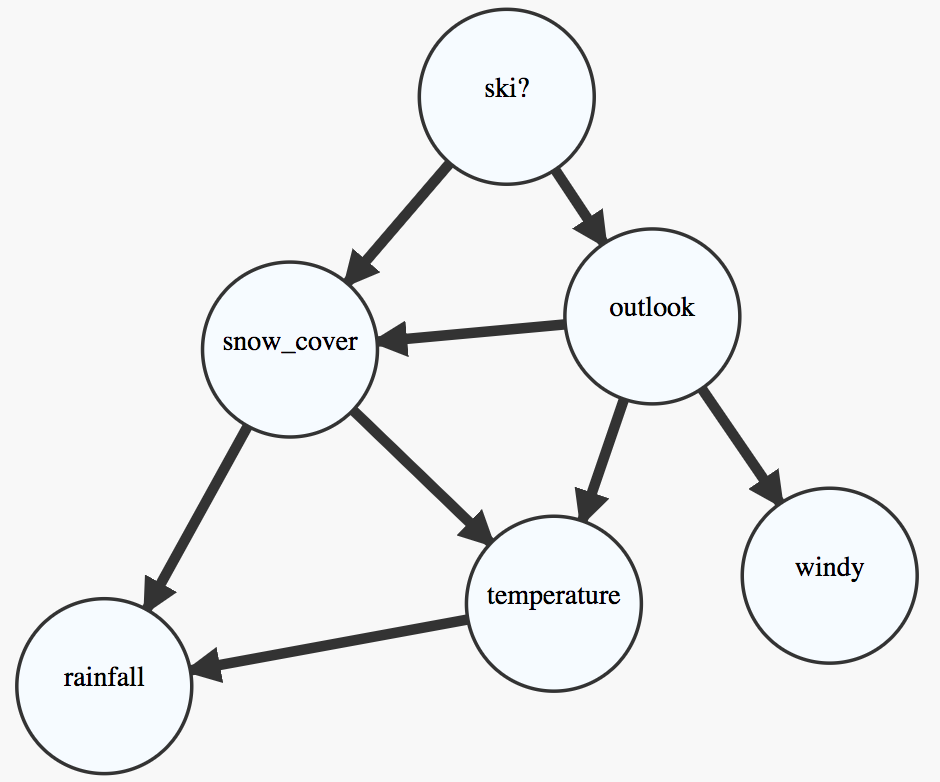
\includegraphics[scale=0.4]{Figures/structure}
\decoRule
\caption{Strucura unei rețele bayesiene}
\label{fig:structure}
\end{figure}

Unul dintre cei mai eficienți algoritmi pentru construirea structurii este algorimul K2, iar pentru calcul costului unui graf în cadrul algorimului de căutare, funcția de scor K2, propusă de Cooper and Herskovits (1992). \cite{carvalho2009scoring}

\subsection{Algoritmul K2}

Algoritmul K2 începe cu o ordine dată a atributelor (noduri) și încearcă să adauge o muchie de la nodurile procesate la cel curent, astfel încât scorul rețelei să fie maxim.

Numărul maxim de părinți poate fi restricționat pentru un nod (la 2 de exemplu) pentru a evita overfitting-ul. În funcția de scor K2 și în calcului tabelelor probabilităților condiționale se poate folosi estimatorul Laplace. \cite{ruiz2005illustration}

În continuare este prezentat algoritmul K2 \cite{cooper1992bayesian}, care caută cea mai probabilă structură a rețelei printr-o metodă euristică, fiind dat un set de cazuri D:

\begin{algorithm}[H]
	\KwData{Un set de n noduri, o ordine a nodurilor, o limită u a numărului de părinți pentru un nod și o bază de date D conținând m cazuri}
	\KwResult{Pentru fiecare nod, un set de părinți}
	\For{$i\leftarrow 1$ \KwTo $n$} {
		$\pi_i \leftarrow \emptyset$\;
		$P_{old} \leftarrow f(i, \pi_i)$ \{Această funcție este calculată folosind ecuația de mai jos\}\;
		$OKToProceed \leftarrow true$\;
		\While{OKToProceed and $|\pi_i| < u$} {
			let $z$ be the node in $Pred(x_i) - \pi_i$ that maximizes $f(i, \pi_i \cup \{z\})$\;
			$P_{new} \leftarrow f(i, \pi_i \cup \{z\})$\;
			\If{$P_{new} > P_{old}$} {
				$P_{old} \leftarrow P_{new}$\;
				$\pi_i \leftarrow \pi_i \cup \{z\}$\;
			}
			\Else {
				OKToPreceed $\leftarrow$ false\;
			}
		}
		write('Node: ', $x_i$, 'Parent of $x_i$: ', $\pi_i$)\;
	}
\end{algorithm}

Ecuația:
\[
	f(i, \pi_i) = \prod_{j=1}^{q_i} \frac{(r_i-1)!}{N_{ij}+r_i-1)!} \prod_{k=1}^{r_i} \alpha_{ijk}!
\]

Unde: \\
$\pi_i$ : setul de părinți pentru nodul $x_i$ \\
$q_i = |\phi_i|$ \\
$\phi_i$ : lista posibilelor instanțe de părinți pentru $x_i$ \\
$r_i = |V_i|$ \\
$V_i$ : lista tuturor valorilor posibile pentru atributul $x_i$ \\
$\alpha_{ijk}$ : numărul de cazuri în D în care atributul $x_i$ este instanțiat cu a $k$-a lui valoare, iar părinții lui $x_i$ în $\pi_i$ sunt instanțiați cu a $j$-a valoare în $\phi_i$ \\
$N_{ij} = \sum_{k=1}^{r_i} \alpha_{ijk}$ : numărul de instanțe din D unde părinții lui $x_i$ în $\pi_i$ sunt instanțiați cu a $j$-a valoare în $\phi_i$
